\documentclass[11pt,a4paper]{article}

\usepackage[a4paper,margin=2.5cm,headheight=14pt,headsep=12pt]{geometry}
\usepackage[T1]{fontenc}
\usepackage[utf8]{inputenc}
\usepackage{lmodern}
\usepackage{microtype}
\usepackage{booktabs}
\usepackage{tabularx}
\usepackage{enumitem}
\usepackage{titlesec}
\usepackage{tcolorbox}
\usepackage{array}
\usepackage{multicol}
\usepackage{fancyhdr}
\usepackage{tikz}
\usepackage{float}
\usepackage{hyperref}
\usepackage{xcolor}
\usetikzlibrary{arrows.meta,positioning}

\definecolor{accent}{RGB}{23,70,115}
\definecolor{rulec}{RGB}{170,190,215}
\definecolor{soft}{RGB}{236,242,249}
\definecolor{warnc}{RGB}{140,40,40}
\definecolor{warnsoft}{RGB}{250,238,238}

\setlength{\parindent}{0pt}
\setlength{\parskip}{6pt}
\setlist{nosep}

\titleformat{\section}{\large\bfseries\color{accent}}{\thesection.}{0.5em}{}
\titlespacing*{\section}{0pt}{16pt}{6pt}

\pagestyle{fancy}
\fancyhf{}
\fancyhead[L]{\small\color{accent}GStar Bootcamp 2026 \,\textperiodcentered\, Individual Project Report}
\fancyhead[R]{\small\color{accent}Van Khue Nguyen}
\renewcommand{\headrulewidth}{0pt}
\fancyfoot[C]{\small\thepage}

\hypersetup{colorlinks=true, linkcolor=accent, urlcolor=accent, citecolor=accent}

\newtcolorbox{hyp}{colback=soft, colframe=accent, boxrule=0.5pt, arc=2pt,
  left=6pt, right=6pt, top=3pt, bottom=3pt}
\newtcolorbox{protocolnote}{colback=warnsoft, colframe=warnc, boxrule=0.5pt, arc=2pt,
  left=6pt, right=6pt, top=3pt, bottom=3pt}

\newcommand{\cell}[1]{\textbf{#1}}

\begin{document}

\begin{center}
  {\LARGE\bfseries\color{accent} Resume or Prevent?}\\[3pt]
  {\large\bfseries Closing Runtime-Transfer Failures in CodeAct Agents: Final Report}\\[5pt]
  {\small Van Khue Nguyen \quad\textperiodcentered\quad École Polytechnique}
\end{center}

\section{Abstract / Project Description}
\label{sec:abstract}

Coding agents built on the CodeAct pattern solve tasks by writing and executing code. They can be
trained under one set of runtime rules and deployed under another. This project studies that
mismatch, together with the two tasks and the four candidate repair levels used throughout
(Section~\ref{sec:problem}). It asks two questions about what actually closes the resulting
quality gap, both decided before running any experiment: whether telling the agent more at
inference time is enough (RQ1), and whether training it differently in the first place does more
(RQ2).

\section{Problem Description and Current Limitations}
\label{sec:problem}

CodeAct agents act by writing one Python block per turn. A per-turn tool-call cap truncates a
block mid-execution, and the unfinished work is lost. An agent fine-tuned on persistent-runtime
traces but deployed on a stateless runtime must rebuild its working record after every reset.

Two CodeAct tasks are used throughout, both procedurally generated with an exact verifier, so no
external data is needed.

\textbf{Opaque Knapsack.} The agent selects a subset of items to maximize total value without
exceeding a weight capacity.
\begin{itemize}
\item \textbf{Tools:}
  \begin{itemize}
  \item \texttt{list\_items()}: returns the candidate item IDs.
  \item \texttt{inspect(item\_id)}: reveals that item's weight, value, and class; spends one
    unit of a limited inspection budget.
  \item \texttt{take(item\_id)}: adds the item, only if its class is allowed and capacity is
    not exceeded.
  \item \texttt{finish()}: ends the episode.
  \end{itemize}
\item \textbf{What ``class'' is for:} only a few classes are allowed per instance, and which
  ones is hidden: \texttt{inspect()} reveals an item's class but not its admissibility. The only
  way to find out is an irreversible \texttt{take()} attempt (safe to reject, but commits the
  item if it succeeds), so the agent must gamble to learn what is even usable \cite{paper}.
\item \textbf{State the agent must track itself:} its running total of weight taken so far (the
  system prompt calls it \texttt{current\_weight}); the environment never reports it back, so a
  mid-turn truncation can wipe it.
\item \textbf{Scoring:} value taken, divided by an exact solver's optimal value; 0 if capacity is
  ever exceeded.
\item \textbf{Config used (the generator's ``medium'' tier, of three):} 40--65 items per
  instance, weight 5--35, value 10--300, drawn from up to 26 classes with only 4 allowed per
  instance; the inspection budget is close to the item count, so the tool-call cap, not the
  inspection budget, is the binding constraint. Every experiment in this project, the RQ1 ladder
  and the RQ2 training/eval pool alike, uses this one tier; easy and hard were never tested.
\end{itemize}

\textbf{Navigation.} The agent moves from a start node to a goal node through a graph it cannot
see in advance.
\begin{itemize}
\item \textbf{Tools:}
  \begin{itemize}
  \item \texttt{neighbors(nodes)}: for up to a fixed number of node IDs per call, reveals what
    each one connects to, plus a hint of whether a needed key is a few hops away.
  \item \texttt{probe(node\_id)}: spends one unit of a limited probe budget to reveal whether
    that node is a trap (teleports the agent elsewhere if stepped on), holds a key, or has an
    outgoing edge locked by some key.
  \item \texttt{move(dst)}: actually steps to an adjacent node.
  \end{itemize}
\item \textbf{How keys and locks relate:} each lock has an ID, and a key only opens edges locked
  with that exact same ID (one key can open several edges if they share a lock ID, but never an
  edge with a different one). Some of the items \texttt{probe()} reports as ``a key'' are decoys
  that do not match any lock at all, included specifically to cost the agent a wasted probe or
  detour.
\item \textbf{State the agent must track itself:} which keys it has already collected and which
  nodes it has already probed; neither is re-surfaced by the environment on request.
\item \textbf{Scoring:} full credit for reaching the goal within the step budget; partial credit
  for ending closer to it than the start.
\item \textbf{Config used (medium tier, same convention as above):} a typical instance has
  around 60 nodes and 100+ edges, a probe budget that reveals only a fraction of the hidden
  structure, 1--2 trap nodes, and 3--5 decoy keys; some goals require collecting more than one
  real key before a locked edge can be crossed.
\end{itemize}

On Opaque Knapsack with Qwen3-8B \cite{paper}, a cap of 25 drops quality from 0.66 (matched
deployment) to 0.07 (mismatched), and a cap of 80 costs $4.4\times$ more tokens (162k vs.\ 37k
per episode). The existing repairs are partial: silent carryover recovers 17\% of the quality
gap; announced carryover cuts post-cap restarts from 0.86 to 0.31 but leaves quality unchanged.
The paper leaves untested whether the agent also needs to know where computation stopped and
what to do next (the paper's own Sec.~6 and App.~E.2 \cite{paper}; this becomes RQ1 below). It
also does not test whether \emph{retraining} the agent to handle the cap differently, rather
than only changing what the runtime shows a fixed agent, closes the gap (RQ2 below, which trains
two different such strategies).

\textbf{The four carryover levels} compared for RQ1 are shown in Figure~\ref{fig:ladder}. L1,
L2, and L3 are mechanically identical: in all three, the cut turn's variables are kept alive for
exactly one more turn. The only thing that differs between them is what the agent is actually
told about that: L1 tells it nothing, L2 names the surviving variables, L3 also reports the last
tool call that completed. This separation is deliberate, so that any score difference between
L1, L2, and L3 can only be attributed to what the agent was told, not to a different amount of
real carryover. (L0 differs mechanically too, keeping nothing at all; it is the no-repair
baseline, not part of that comparison.)

\begin{figure}[H]
\centering
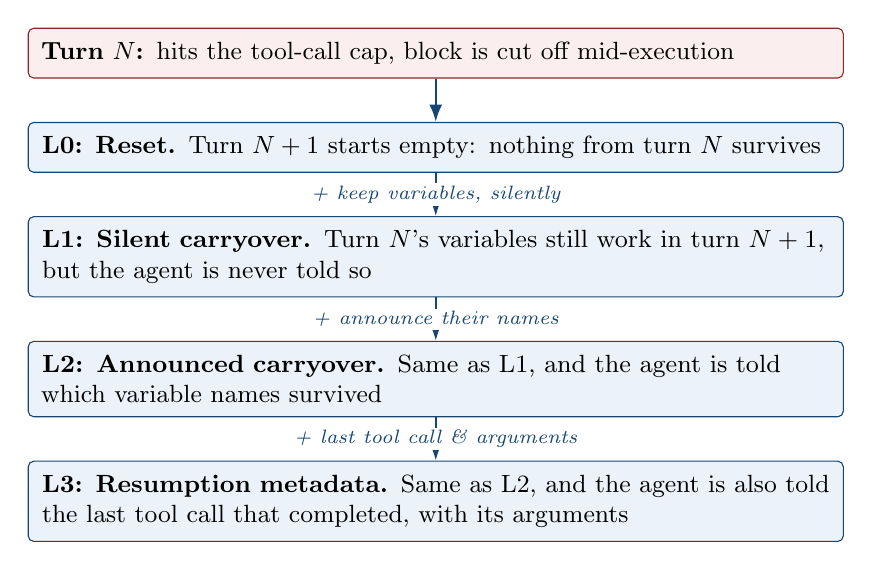
\begin{tikzpicture}[
  box/.style={draw=accent, rounded corners=2pt, fill=soft, align=left, font=\small,
    text width=10cm, inner sep=5pt},
  cutbox/.style={draw=warnc, rounded corners=2pt, fill=warnsoft, align=left, font=\small,
    text width=10cm, inner sep=5pt},
  arr/.style={-{Latex[length=2.2mm]}, accent, thick},
  lbl/.style={font=\scriptsize\itshape, text=accent, fill=white, inner sep=1pt}
]
\node[cutbox] (cut) {\textbf{Turn $N$:} hits the tool-call cap, block is cut off mid-execution};
\node[box, below=0.55cm of cut] (l0) {\textbf{L0: Reset.} Turn $N+1$ starts empty: nothing from turn $N$ survives};
\node[box, below=0.55cm of l0] (l1) {\textbf{L1: Silent carryover.} Turn $N$'s variables still work in turn $N+1$, but the agent is never told so};
\node[box, below=0.55cm of l1] (l2) {\textbf{L2: Announced carryover.} Same as L1, and the agent is told which variable names survived};
\node[box, below=0.55cm of l2] (l3) {\textbf{L3: Resumption metadata.} Same as L2, and the agent is also told the last tool call that completed, with its arguments};
\draw[arr] (cut) -- (l0);
\draw[arr] (l0.south) -- node[lbl]{+ keep variables, silently} (l1.north);
\draw[arr] (l1.south) -- node[lbl]{+ announce their names} (l2.north);
\draw[arr] (l2.south) -- node[lbl]{+ last tool call \& arguments} (l3.north);
\end{tikzpicture}
\caption{The four carryover levels evaluated for RQ1. L1--L3 all keep the identical real
carryover (one extra turn of the cut block's variables); only what the runtime tells the agent
about it changes.}
\label{fig:ladder}
\end{figure}

\textbf{RQ1.} Does showing the agent explicit resumption metadata (the last completed tool call
and its arguments), on top of announced carryover, recover more quality than announced carryover
alone? Answered in two steps: first, by re-running the L3-vs-L2 comparison on 50 held-out
instances and then re-running the exact same comparison several more times, changing only the
wording of the metadata banner, to check whether the result holds up or was a fluke of one
particular phrasing. Second, by a separate experiment (Section~\ref{sec:mechanism}) that checks
whether the agent's problem is really a lack of information, as RQ1 assumes, or something else.

\textbf{RQ2.} Does training an adapter on a prevention-style strategy (avoid truncation in the
first place) outperform one trained on a recovery-style strategy (resume from metadata after
being truncated), at matched tool calls and trace length? Answered by generating teacher traces
for both strategies, pairing and filtering them as in the paper's own methodology, training two
QLoRA adapters, and evaluating both on the same 50 held-out instances across two cap settings (a
tight cap and a slack cap), with a rule fixed before training to scale up the training data if
the first pass showed no signal.

\section{RQ1 Results: Resumption Metadata vs.\ Announced Carryover}
\label{sec:rq1}

\textbf{Setup.} 50 held-out Opaque Knapsack instances (seed\_start 91000, disjoint from the
paper's own 25-instance eval set and from every training pool used anywhere in this project;
see Section~\ref{sec:data}), trained persistent and deployed stateless (P$\to$S), cap 25,
Qwen3-8B persistent-trained adapter, the four levels defined in Figure~\ref{fig:ladder}. Every
comparison below is a paired bootstrap over these same 50 instances (10,000 resamples); ``sig.''
means the resulting 95\% confidence interval excludes zero, ``ns'' (not significant) means it
includes zero.

\begin{table}[H]
\centering
\small
\begin{tabular}{@{}lrr@{}}
\toprule
\cell{Condition} & \cell{Mean score} & \cell{Tokens / episode} \\
\midrule
L0 Reset & 0.025 & 490k \\
L1 Silent carryover & 0.165 & 443k \\
L2 Announced carryover & 0.122 & 480k \\
L3 Resumption metadata & 0.235 & 420k \\
\bottomrule
\end{tabular}
\caption{Mean score and mean token cost by carryover level, on the same 50 held-out instances.
These are large numbers because every condition here is the \emph{mismatched} case (a
persistent-trained adapter deployed stateless): rebuilding lost context repeatedly is expensive,
the same pattern the paper itself reports.}
\label{tab:ladder-scores}
\end{table}

The rerun check in Table~\ref{tab:wording} shows that cost is just as unstable as score. With
nothing changed at all, L2's token cost moved from 480k to 420k and L3's moved from 420k to 381k
between the original run and its plain rerun. If a single run's score cannot be trusted on its
own (Section~\ref{sec:rq1}'s whole point), neither can its token cost.

\begin{table}[H]
\centering
\small
\begin{tabular}{@{}lrll@{}}
\toprule
\cell{Comparison} & \cell{Diff} & \cell{95\% CI} & \\
\midrule
L1$-$L0 & $+0.140$ & $[+0.065,+0.224]$ & sig. \\
L2$-$L1 & $-0.043$ & $[-0.140,+0.053]$ & ns \\
L3$-$L2 (\textbf{the RQ1 test}) & $+0.113$ & $[+0.009,+0.217]$ & sig.\ (first run only; see below) \\
L3$-$L1 & $+0.071$ & $[-0.047,+0.186]$ & ns \\
L3$-$L0 & $+0.210$ & $[+0.115,+0.309]$ & sig. \\
\bottomrule
\end{tabular}
\caption{Pairwise comparisons between the levels in Table~\ref{tab:ladder-scores}. The RQ1
test, decided before seeing any results, is L3$-$L2: does resumption metadata beat announced
carryover.}
\label{tab:ladder-pairs}
\end{table}

Looking only at this one result (Table~\ref{tab:ladder-pairs}'s L3$-$L2 row), resumption
metadata beats announced carryover, exactly what RQ1 predicted. \textbf{To check whether that
holds up, the same comparison was investigated further.} ``Original'' is the plain L3 banner as
specified in Figure~\ref{fig:ladder}: just the variable names and the last tool call, with no
further explanation of what to do with them. The comparison was re-run four more times on the
same 50 instances. The first rerun is a rerun of Original itself, with nothing changed at all:
same banner, same wording, same instances, run again from scratch, to measure how much the
result moves from run-to-run noise alone, with no wording difference to blame it on. The other
three each add a different kind of explanatory text on top of that same banner, to see whether
explaining the information helps the agent put it to use:
\begin{itemize}
\item \textbf{A short added rule} (``note''): one or two extra sentences, added once to the
  system prompt and present identically on every turn.
\item \textbf{Shown only when relevant} (``inline''): the same kind of sentence, but inserted
  only into the specific turn's own observation, on the turn it actually applies to, instead of
  sitting in the prompt the whole time.
\item \textbf{A worked example} (``few-shot''): a 3-turn example conversation, placed in the
  prompt before the task starts and shown once per episode, demonstrating hitting the cap,
  correctly reusing the carried variable, then redeclaring it.
\end{itemize}

\begin{table}[H]
\centering
\small
\begin{tabular}{@{}lrrrl@{}}
\toprule
\cell{Banner wording variant} & \cell{L2 mean} & \cell{L3 mean} & \cell{diff} & \cell{95\% CI (L3$-$L2)} \\
\midrule
Original (reported above)             & 0.122 & 0.235 & $+0.113$ & $[+0.009,+0.217]$ \quad\textbf{sig.} \\
Original, rerun (nothing changed)     & 0.216 & 0.232 & $+0.017$ & $[-0.095,+0.136]$ \quad ns \\
Added rule (``note'')                 & 0.124 & 0.173 & $+0.049$ & $[-0.064,+0.160]$ \quad ns \\
Shown only when relevant (``inline'') & 0.108 & 0.092 & $-0.016$ & $[-0.101,+0.062]$ \quad ns \\
Worked example (``few-shot'')         & 0.223 & 0.233 & $+0.010$ & $[-0.112,+0.137]$ \quad ns \\
\bottomrule
\end{tabular}
\caption{The same L3$-$L2 comparison as Table~\ref{tab:ladder-pairs}, repeated four more times:
first a plain rerun of Original with nothing changed, then three wording variants. Only the
original run is nominally significant, including against its own rerun.}
\label{tab:wording}
\end{table}

This investigation shows the original result does not persist: only 1 of the 5 attempts is
nominally significant, and the spread across attempts ($-0.02$ to $+0.11$)
is larger than the paper's own documented rerun noise (the paper's own App.~F.2
\cite{paper}: 0.057 mean absolute shift between two repeated rollouts of the same adapter, with
nothing else changed at all). The plain rerun is the clearest point: L2's own mean score moved
from 0.122 to 0.216, nearly doubling, with the prompt held completely fixed. \textbf{Conclusion:
RQ1 is not supported.} Resumption metadata does not reliably beat announced carryover at this
sample size, and the instability is not a wording artifact: it is present even when nothing is
changed at all. A single favorable-looking result, among several equally reasonable ways of
running the same comparison (wording changed or not), is not evidence by itself; this is exactly
why it was checked against the others before being trusted.

\begin{protocolnote}
\textbf{Protocol note: a planning mistake, found and fixed.} The original project proposal set a
rule: train the recovery strategy only if resumption metadata (L3) already beats announced
carryover (L2) \emph{without} any training, i.e., only if RQ1 succeeds on its own first. That
rule rests on a mistake. RQ1 tests whether an \emph{untrained} model can use resumption metadata
by itself; RQ2 tests whether a model can be \emph{trained} to use it. These are different
skills, so failing at the first does not mean failing at the second. RQ1's null result
(Section~\ref{sec:rq1}) was therefore never actually a reason to skip training the recovery
strategy, and it was trained anyway. This note explains why that was the right call, even though
the plan as originally written in the proposal said otherwise.
\end{protocolnote}

\section{Mechanism: The Trap Is a Training-Time Prior, Not an Information Gap}
\label{sec:mechanism}

Section~\ref{sec:rq1} only showed \emph{that} giving the agent more information does not
reliably help. This section asks \emph{why}, by looking at what the agent actually does turn by
turn, not just its final score.

\textbf{Design.} A $2\times2$ experiment, on two more seeds (1337, 777; $n=50$ each), crosses two
things that are normally tangled together: which runtime the agent was \emph{trained} on
(persistent vs.\ stateless) against how much it is \emph{told} at test time (L1 silent vs.\ L2
announced). Every combination is deployed on the same stateless runtime at test time: this is
the mismatched condition for the persistent-trained adapter (same P$\to$S setup as RQ1), and the
matched condition for the stateless-trained one, which is by design, not an oversight: it is
exactly what lets the comparison isolate training. If the failure were really an information
gap, telling either adapter more (L2) should help regardless of which one it is. If it is a
trained habit instead, only the mismatched (persistent-trained) adapter should show it, since
the matched one never had a reason to learn that habit in the first place.

Two concrete, per-turn behaviors are measured, not just the final score:

\textbf{Trap rate.} A cap-cut keeps certain variables alive for exactly one more turn
(Figure~\ref{fig:ladder}). The trap is springing this specifically \emph{two} turns after the
cut, once that one-turn grant has already expired. Trap rate is the share of such opportunities
(a turn that was not itself cut, with a following turn to check) where this actually happens.

\begin{hyp}
\textbf{A real example} (persistent-trained adapter, L2, one episode). Turn 0 is cut mid-block
with \texttt{to\_inspect} (among others) still alive. Turn 1 correctly reuses
\texttt{to\_inspect[:25]}, within its one-turn grant, and succeeds. Turn 2 refers to
\texttt{to\_inspect[25:52]} again, one turn past its grant: \texttt{NameError: name
'to\_inspect' is not defined}. That is one trap hit, caught in the trace rather than only in the
aggregate rate below.
\end{hyp}

\textbf{Fabrications.} \texttt{inspect()} is the only legitimate source of an item's real value
and weight. A fabrication is the agent's code asserting a specific, wrong value or weight for a
real item id, for example writing down \texttt{\{"item\_4f2": \{"value": 90, "weight": 12\}\}}
when that item's real value is 140, counted once per item per task even if the same wrong number
is repeated across several turns. This flags any wrong value, whether invented outright or a
real one copied down incorrectly; it does not try to tell those two apart (Section~\ref{sec:limitations}).

\begin{table}[H]
\centering
\small
\begin{tabular}{@{}llrrr@{}}
\toprule
\cell{Training regime} & \cell{Level} & \cell{Score} & \cell{Trap rate} & \cell{Fabrications / 50 tasks} \\
\midrule
Persistent, seed 1337 & L1 & 0.073 & 74.0\% (97/131) & 0 \\
Persistent, seed 1337 & L2 & 0.215 & 58.4\% (142/243) & 0 \\
Persistent, seed 777  & L1 & 0.071 & 62.3\% (81/130)  & 0 \\
Persistent, seed 777  & L2 & 0.213 & 67.8\% (187/276) & 0 \\
Stateless, seed 1337  & L1 & 0.268 & 0\% (0/38)        & 155 \\
Stateless, seed 1337  & L2 & 0.250 & 0\% (0/40)        & 452 \\
Stateless, seed 777   & L1 & 0.264 & 0\% (0/37)        & 60 \\
Stateless, seed 777   & L2 & 0.313 & 0\% (0/47)        & 430 \\
\midrule
Base model, no LoRA & L1 & 0.014 & 86.7\% (26/30) & 1 \\
Base model, no LoRA & L2 & 0.018 & 66.2\% (43/65) & 0 \\
\bottomrule
\end{tabular}
\caption{The persistent/stateless $\times$ L1/L2 ablation, two seeds, 50 instances each. Trap
rate = share of cap-cut opportunities where the next-next turn hits a \texttt{NameError} on a
carried variable.}
\label{tab:mechanism}
\end{table}

The pattern is consistent across both seeds and both carryover levels: \textbf{persistent-trained
models fall into the trap 58--74\% of the time no matter whether the carried names are announced
(L2) or not (L1); stateless-trained models never fall into it (0\%), at either level}. Announcing
what is available does not move the persistent model's trap rate; the behavior is a prior
learned from training on a runtime where variables always persist, not a response to missing
information in the prompt. This is also why RQ1's fix (more information) could not reliably
work: the failure it targets is not an information deficit.

The two training regimes trade one failure for another: stateless training removes the trap but
introduces real, substantial fabrication (60--452 wrong item claims across 50 tasks): the
model, never having had carryover to rely on, guesses item values it never inspected. Persistent
training never fabricates (0 in all four cells) but traps instead. Neither failure mode is fixed
by changing what the runtime announces; both are set by what the model was trained on.

\textbf{A cross-domain check on Navigation.} Section~\ref{sec:rq1}'s central question, whether
\emph{explaining} more to the agent helps beyond just giving it real information, is tested
again here: on a structurally different task (Section~\ref{sec:problem}), using the same L0--L3
ladder (Figure~\ref{fig:ladder}), on 50 fresh, independently-generated instances.

\begin{table}[H]
\centering
\small
\begin{tabular}{@{}lrrll@{}}
\toprule
\cell{Condition} & \cell{Mean score ($n=50$)} & \cell{Comparison} & \cell{Diff} & \cell{95\% CI} \\
\midrule
L0 (reset)                  & 0.336 & -- & -- & -- \\
L1 (silent carryover)       & 0.258 & L1 $-$ L0 & $-0.077$ & $[-0.225,+0.072]$ \quad ns \\
L2 (announced carryover)    & 0.386 & L2 $-$ L0 & $+0.051$ & $[-0.083,+0.187]$ \quad ns \\
L3 (resumption metadata)    & 0.291 & L3 $-$ L0 & $-0.045$ & $[-0.160,+0.071]$ \quad ns \\
                             &       & L2 $-$ L1 & $+0.128$ & $[+0.018,+0.240]$ \quad\textbf{sig.} \\
                             &       & L3 $-$ L2 & $-0.096$ & $[-0.232,+0.036]$ \quad ns \\
\bottomrule
\end{tabular}
\caption{The full L0--L3 comparison on Navigation, on 50 fresh, non-overlapping instances
(disjoint seed pool, no instance reused from any other table in this report).}
\label{tab:nav-rep50}
\end{table}

This pattern is unstable, and no single level can be called reliably better. Only one of the
five comparisons is significant (L2$-$L1), and it is the narrowest kind of comparison in this
report, the same kind that evaporated under a rerun in Knapsack (Table~\ref{tab:wording}). More
to the point: \emph{nothing here reliably beats doing nothing}. L1, L2, and L3 are all
statistically indistinguishable from L0. This does not match Knapsack, where real carryover
clearly beat no carryover at all (Table~\ref{tab:ladder-pairs}). Navigation does not confirm
Knapsack's result; it is an independent test, and it came out differently.

\textbf{Two further, more targeted ablations.} Navigation's default L2/L3 prompt already
includes a worked example demonstrating how to use the carryover information; for L3, that
example explicitly explains why \texttt{last\_action} matters (\textit{``I'll look up that exact
node\ldots which is the whole reason this field exists''}). Two ablations isolate what is
actually doing the work inside that prompt. The first separates the worked example from the real
announcement: removing the example from L2, and separately adding it to L1 without any real
announcement, asks whether the \emph{example} or the \emph{real information} is doing the work.
The second keeps everything about L3 intact, including that same worked example explaining
\texttt{last\_action}, but blanks out \texttt{last\_action}'s real value at runtime, asking
whether being explicitly taught that a field matters translates into it actually helping.

These two ablations were run on the same 50-instance independent pool as the main comparison
above (Table~\ref{tab:nav-rep50}), not a smaller or separately-pooled design.

\begin{table}[H]
\centering
\small
\begin{tabular}{@{}lrll@{}}
\toprule
\cell{Comparison} & \cell{Diff} & \cell{95\% CI} & \\
\midrule
(L2, example removed) $-$ L2 & $-0.052$ & $[-0.157,+0.048]$ & ns \\
(L1, example added) $-$ L1 & $+0.015$ & $[-0.096,+0.129]$ & ns \\
(L1, example added) $-$ (L2, example removed) & $-0.061$ & $[-0.173,+0.055]$ & ns \\
L3 $-$ (L3, \texttt{last\_action} blanked) & $-0.021$ & $[-0.153,+0.114]$ & ns \\
\bottomrule
\end{tabular}
\caption{The two ablations described above, paired bootstrap on the same 50-instance
independent pool as Table~\ref{tab:nav-rep50}.}
\label{tab:nav-ablation}
\end{table}

Both ablations are null too: separating the worked example from the real announcement does not
reliably move the score either way, so the two cannot be told apart at this $n$; and even though
the agent is explicitly taught why \texttt{last\_action} matters, blanking out its real value
does not reliably hurt the score. Taken together, Navigation does not give this report a second
task to confirm Knapsack's story on. It gives a second, independent result, and that result is
mostly null and does not match the first.

\section{RQ2 Results: Training on a Strategy}
\label{sec:rq2}

\textbf{Setup.} Gemini 3 Flash teacher traces are generated at cap 25, on the stateless runtime,
with the metadata banner present for both strategies:
\begin{itemize}
\item \textbf{Prevention:} each block is capped below the tool-call limit, with a mandatory
  progress checkpoint at the end of it, so the teacher is never actually truncated.
\item \textbf{Recovery:} blocks are unrestricted; after a truncation, the metadata banner is
  shown, and the trace is kept only if the teacher actually resumes correctly from it.
\end{itemize}

\begin{hyp}
\textbf{A real example} (recovery adapter, cap 25, one episode). The agent's block is cut
mid-way through taking items. The runtime's own banner for the next turn reports
\texttt{last\_action: \{tool: inspect, args: [item\_c8ccbaf59ab0]\}}, the last tool call that
completed before the cut. The agent's very next turn opens with: \textit{``I will now resume
from the last successful action (\texttt{inspect("item\_c8ccbaf59ab0")})\ldots''}, naming the
exact tool and argument the banner reported. This is not a coincidence: the agent is reading the
resumption metadata and using it, the behavior recovery's training is meant to produce.
\end{hyp}

Instances are paired and filtered exactly as in the paper's own Appendix B \cite{paper}.
Concretely (\texttt{train/prepare\_paired\_data.py}, \texttt{train/trace\_validator.py} in the
code release): for a given instance, both its prevention trace and its recovery trace are
checked against the same four criteria: a score of at least 0.5; \texttt{finish()} called
within the last 3 steps; no near-duplicate loop (the final assistant message is not more than
90\% similar to 3 of the last 4); and an error rate at or below 10\%, not counting the
tool-call-limit and ``class not allowed'' errors the model is specifically meant to learn to
handle. An instance is kept only if \emph{both} traces pass all four checks, so the two adapters
are trained on the exact same set of instances, not two different ones.

\textbf{Training recipe.} Two QLoRA adapters are trained per scale, using the paper's own
recipe except for one change applied to both (Table~\ref{tab:hparams}): effective batch size,
reduced from 16 to 4, decided before training.

\begin{table}[H]
\centering
\small
\begin{tabular}{@{}ll@{}}
\toprule
\cell{Hyperparameter} & \cell{Value} \\
\midrule
LoRA rank & 64 \\
LoRA alpha & 128 \\
LoRA dropout & 0.05 \\
Learning rate & $10^{-4}$, cosine schedule \\
Epochs & 3 \\
Sequence length & 16{,}384 tokens \\
Effective batch size & \textbf{4} (paper's own recipe: 16) \\
\bottomrule
\end{tabular}
\caption{QLoRA recipe for the prevention/recovery adapters. Every value is the paper's own
recipe, unchanged, except effective batch size (bold).}
\label{tab:hparams}
\end{table}

\textbf{Why.} At the paper's batch 16, 56 pairs over 3 epochs gives only 12 optimizer steps on
an 8B model, too few to tell ``no effect'' from ``no training.'' At batch 4 this is 42 steps
($n=56$) or 75 ($n=100$). The same change applies to both adapters, so it cannot bias the
comparison between them.

Both adapters are evaluated $2\times2$ (strategy $\times$ cap $\{25,80\}$) on the same 50
held-out instances used throughout this report.

\begin{table}[H]
\centering
\small
\begin{tabular}{@{}lrr|rr@{}}
\toprule
 & \multicolumn{2}{c}{\cell{$n=56$ pairs (40 steps)}} & \multicolumn{2}{c}{\cell{$n=103$ pairs (74 steps)}} \\
\cmidrule(lr){2-3} \cmidrule(lr){4-5}
 & cap 25 & cap 80 & cap 25 & cap 80 \\
\midrule
Prevention mean   & 0.234 & 0.381 & 0.537 & 0.555 \\
Recovery mean     & 0.194 & 0.304 & 0.275 & 0.481 \\
Diff (Prev$-$Rec) & $+0.040$ & $+0.077$ & $+0.262$ & $+0.074$ \\
95\% CI           & $[-0.079,+0.157]$ & $[-0.060,+0.207]$ & $\mathbf{[+0.141,+0.382]}$ & $[-0.057,+0.197]$ \\
CI width          & 0.236 & 0.266 & 0.241 & 0.254 \\
\bottomrule
\end{tabular}
\caption{Prevention vs.\ recovery, at both training scales and both caps, on the same 50
held-out instances.}
\label{tab:rq2-main}
\end{table}

Per the rule fixed in advance (``grow toward $\sim$100 pairs only if the 56-pair run
shows no signal''), the 56-pair null triggered the scale-up to 103 pairs. \textbf{RQ2 is now
supported at cap 25} (first CI in this project excluding zero) and \textbf{remains a null at cap
80}, and the gap shrinking at the slack cap is exactly what the proposal predicted in advance.
Notably, the CI width barely changed (cap 25: $0.236\to0.241$); what changed was the point
estimate. More data did not make the measurement more precise so much as it let both adapters
finish learning the behavior at all (74 real optimizer steps vs.\ 40 on an otherwise-identical
8B QLoRA recipe): the 56-pair run was closer to undertrained than to a tight null.

\textbf{Unlike RQ1's apparent win, this one survives a plain rerun.} The same eval, on the same
$n=103$ adapters, nothing changed, was run again from scratch. Cap 25: $+0.240$, CI
$[+0.102,+0.375]$, still significant. Cap 80: $+0.018$, CI $[-0.096,+0.129]$, still null. Both
land close to the original numbers above. This is the same check that showed RQ1's L3$-$L2 win
could not be trusted on its own (Table~\ref{tab:wording}); run here, it comes back clean.

Section~\ref{sec:mechanism}'s other failure mode, the carryover trap, was also checked on these
same traces and is not relevant here: trap hits are 0 in every one of the four cells, including
at cap 25 where real cap-cut opportunities do occur (93 of them for recovery alone). This is
consistent with that section's own finding that the trap is specific to persistent-trained
models; neither prevention nor recovery was trained that way, so there is no persistent-training
prior for it to come from. A test-time fabrication check on these same adapters' eval traces
gives a mechanistic reason specific to cap 25:

\begin{table}[H]
\centering
\small
\begin{tabular}{@{}lrr@{}}
\toprule
\cell{Cell ($n=103$ adapters)} & \cell{Tasks with $\geq$1 fabrication / 50} & \cell{Total fabricated items} \\
\midrule
Prevention, cap 25 & 0 & 0 \\
Recovery, cap 25   & 2 & 20 \\
Prevention, cap 80 & 0 & 0 \\
Recovery, cap 80   & 0 & 0 \\
\bottomrule
\end{tabular}
\caption{Fabrication at test time, on the $n=103$ adapters' own eval traces.}
\label{tab:rq2-fab}
\end{table}

Fabrication at test time appears only for recovery at cap 25, the one cell where recovery
also loses on score, and is absent everywhere prevention is used and everywhere the cap is
slack. A plausible mechanism, not confirmed beyond these two episodes: recovery's whole design
depends on resuming correctly after a truncation, and when that resumption does not land
exactly right, the model may guess a value to keep going rather than stop, something
prevention's design never puts it in a position to do, since it is never truncated in the first
place.

This is a different, and more informative, check than comparing the \emph{teacher} traces used
for training: both strategies' teacher traces show zero fabrication, since Gemini 3 Flash rarely
fabricates under this prompt regardless of strategy. The effect is specific to what the smaller,
cap-pressured 8B student does at test time, not to what it was shown during training.

\textbf{When does prevention win, and at what cost?} Not just on average, and not only on a few
tasks. Counting task by task instead of averaging: at cap 25, prevention beats recovery outright
on 34 of the 50 held-out tasks, loses on 12, and ties on 4. At cap 80, where
Table~\ref{tab:rq2-main}'s \emph{average} difference is null, prevention still wins more tasks
than it loses, 30 to 14 (6 ties); a null average can still hide a lopsided win count, and here it
does.

Is the win concentrated on easier or harder tasks? Splitting the 50 instances in half by size
(more items vs.\ fewer), prevention is ahead in both halves (+0.33 on the smaller-instance half,
+0.19 on the larger-instance half), and the size of an instance barely predicts which strategy
wins it. So the advantage looks broad, not a few easy wins padding the average.

Prevention is also the cheaper strategy. At cap 25, recovery spends 183k tokens and 12.3 turns
per episode on average, against prevention's 107k tokens and 8.7 turns, about 70\% more. This
follows directly from what each strategy does: recovery has to resume from a cut, which costs
extra turns and tokens, while prevention is designed never to be cut in the first place. At cap
80 the gap narrows but recovery is still pricier (129k vs.\ 97k tokens). Prevention wins on
quality at the tight cap, and on cost at both caps.

\section{Conclusion}
\label{sec:conclusion}

Put together: telling a mismatched agent more does not reliably help; retraining it to behave
differently under the cap does, specifically where the cap is tight enough to matter.

\textbf{RQ1 is a demonstrated null, not an unexamined one.}
\begin{itemize}
\item The apparent win from resumption metadata (L3$-$L2, $+0.113$, sig.) does not persist: only
  1 of 5 reruns (the original plus 4 reruns, one of them a plain rerun with nothing changed) is
  nominally significant, and the spread across them ($-0.02$ to $+0.11$) exceeds the paper's own
  documented rerun noise.
\item The null is explained by a mechanism, not left unexplained: the 2$\times$2 check
  (Section~\ref{sec:mechanism}) shows the carryover trap is a property of what runtime the model
  was \emph{trained} on, not of what the prompt announces.
\item A cross-domain check on Navigation ($n=50$) does not confirm Knapsack's result. No
  carryover level there reliably beats doing nothing, and the one significant comparison found
  is the narrowest kind this report has, the same kind that proved fragile under rerun
  elsewhere.
\end{itemize}

\textbf{RQ2 is a real, modest positive result.}
\begin{itemize}
\item Supported at cap 25 ($n=103$): prevention beats recovery by $+0.262$, CI excluding zero,
  and this one holds up under a plain rerun ($+0.240$, still significant), unlike RQ1's.
\item Null at cap 80, matching the direction predicted in advance: the gap should shrink, and
  does, once the cap is slack enough that the underlying failure stops biting.
\item Backed by a matching test-time fabrication signal: recovery fabricates item values only in
  the one cell where it also loses on score (cap 25), and never where the cap is slack or where
  prevention is used.
\end{itemize}

\section{What Changed From the Proposal}
\label{sec:changes}

\begin{itemize}
\item \textbf{Scale-up, per the rule fixed in advance.} 56$\to$103 training pairs (180 raw
  instances, 57.2\% valid-pair yield, matching the paper's own 58.4\%), triggered because the
  56-pair run showed no signal, exactly as planned in advance.
\item \textbf{One further repair level, proposed as a stretch goal, was not attempted, for lack
  of time:} giving the agent a saved snapshot of the truncated block's own state, rather than
  just announcing which variables survived. (A second level, having the runtime silently resume
  the cut block itself, was never in scope: the proposal itself flagged it as not feasible
  without changing how the cap is accounted for.)
\item \textbf{The recovery-branch contingency deviation} is disclosed in Section~\ref{sec:rq1}'s protocol
  note.
\end{itemize}

\section{Data, Code, and Reproducibility}
\label{sec:data}

\begin{itemize}
\item \textbf{Code and report:}
  \url{https://github.com/TieuDaoChanNhan/resume-or-prevent} (the configs, benchmark, and
  training code for every cell reported here, including the reruns in Sections~\ref{sec:rq1}
  and~\ref{sec:mechanism}); \texttt{report/} holds this PDF and its \LaTeX{} source.
\item \textbf{Raw traces and checkpoints:} the prevention/recovery adapters (both scales) are
  released as four separate model repos, and every raw trace this project generated (the
  Knapsack rerun, the Navigation replication and ablations, the RQ2 training and evaluation
  traces) as one dataset repo, both under the \texttt{TieuDaoChanNhan} account and grouped into
  one collection: \href{https://huggingface.co/collections/TieuDaoChanNhan/resume-or-prevent-gstar-2026-individual-project-6adf7ab692e0177bc1477d73}{huggingface.co/TieuDaoChanNhan (collection)}.
  The mechanistic 2$\times$2 (Section~\ref{sec:mechanism}) reuses the paper's own already-released
  Knapsack and Navigation adapters directly; those are not duplicated here.
\end{itemize}

\section{Limitations}
\label{sec:limitations}

\begin{itemize}
\item $n=103$ pairs is far below the paper's own $n=1000$/side; the cap-25 RQ2 result is a single
  train/eval run at this scale, not a seed-replicated one (unlike the RQ1 ladder work in Section~\ref{sec:rq1},
  which used 2--3 seeds throughout).
\item The trap-rate and fabrication detectors (Section~\ref{sec:mechanism}) are regex-based
  heuristics, not a semantic check, written for this project and tested against synthetic traces
  before use. Both are biased toward under-counting, not over-counting: the fabrication detector
  only flags a value after checking it against the task's real ground truth, and the trap
  detector excludes built-in/generic variable names and fresh redeclarations by construction, so
  neither can report a false positive, only miss a real one phrased outside the pattern it looks
  for. Both are plausible lower bounds on the true rate.
\item Both RQs are studied only on Opaque Knapsack (RQ2) or Knapsack plus Navigation (RQ1); generalization to other CodeAct tasks is untested.
\end{itemize}

\section{Brief Literature Review}
\label{sec:litreview}

\textbf{Foundation.} The setting is the IAEval 2026 paper \cite{paper}, which builds on CodeAct
\cite{codeact}. (CodeACT \cite{codeact2} is a different paper with the same acronym; it is not
used here.)

\textbf{Memory and summarization.} MemGPT \cite{memgpt}, Mem1 \cite{mem1}, and ReSum
\cite{resum} keep state available across turns. To our knowledge, none studies what an agent
must know to resume an interrupted block. This project's negative result on RQ1 suggests the
relevant gap for this family of failures is training exposure, not in-context state access.

\textbf{Budget and asynchrony (adjacent).} Budget-aware tool use \cite{budget}, BAGEN
\cite{bagen}, AsyncTool \cite{asynctool}, and Gaia2 \cite{gaia2} study budgets or delayed tool
feedback. This project studies a mismatch between training and deployment contracts instead.

\section{Contribution Statement}
\label{sec:contribution}

This is an individual project. It builds on the released code, traces, and adapters of the paper
\cite{paper} (Apache-2.0, public on Hugging Face), and on its silent and announced carryover
results.

My contributions:
\begin{itemize}
\item \textbf{(i) RQ1:} the resumption-metadata runtime condition itself, plus its wording and
  cross-domain robustness checks (Section~\ref{sec:rq1}).
\item \textbf{(ii) Mechanism:} the 2$\times$2 and cross-domain ablations tracing the carryover
  trap to a training-time habit, not a gap in what the prompt says (Section~\ref{sec:mechanism}).
\item \textbf{(iii) RQ2:} building, training, and scaling up, by a rule fixed in advance, the
  prevention and recovery adapters, and evaluating them head-to-head at two caps
  (Section~\ref{sec:rq2}).
\end{itemize}

The paper leaves both (i) and (iii) open: whether more information helps without retraining, and
whether retraining helps at all. (ii) connects them: it is why (i) and (iii) answer differently,
tested directly rather than assumed.

\small
\begin{thebibliography}{9}
\bibitem{paper} Victor May, Van Khue Nguyen, Aaditya Salgarkar, Yishan Wang, Diganta Misra, and Huu Nguyen. \emph{Evaluating Agents Across Runtime Contracts: When Mismatch Costs Efficiency or Quality}. arXiv:2603.01209, IAEval 2026. \url{https://arxiv.org/abs/2603.01209}
\bibitem{codeact} Xingyao Wang, Yangyi Chen, Lifan Yuan, Yizhe Zhang, Yunzhu Li, Hao Peng, and Heng Ji. \emph{Executable Code Actions Elicit Better LLM Agents}. ICML 2024. arXiv:2402.01030. \url{https://arxiv.org/abs/2402.01030}
\bibitem{codeact2} Weijie Lv, Xuan Xia, and Sheng-Jun Huang. \emph{CodeACT: Code Adaptive Compute-efficient Tuning Framework for Code LLMs}. arXiv:2408.02193, 2024. \url{https://arxiv.org/abs/2408.02193}
\bibitem{memgpt} Charles Packer, Sarah Wooders, Kevin Lin, Vivian Fang, Shishir G. Patil, Ion Stoica, and Joseph E. Gonzalez. \emph{MemGPT: Towards LLMs as Operating Systems}. arXiv:2310.08560, 2023. \url{https://arxiv.org/abs/2310.08560}
\bibitem{mem1} Zijian Zhou, Ao Qu, Zhaoxuan Wu, Sunghwan Kim, Alok Prakash, Daniela Rus, Bryan Kian Hsiang Low, and Paul Pu Liang. \emph{MEM1: Learning to Synergize Memory and Reasoning for Efficient Long-Horizon Agents}. ICLR 2026. arXiv:2506.15841. \url{https://arxiv.org/abs/2506.15841}
\bibitem{resum} Xixi Wu, Kuan Li, Yida Zhao, et al. \emph{ReSum: Unlocking Long-Horizon Search Intelligence via Context Summarization}. arXiv:2509.13313, 2025. \url{https://arxiv.org/abs/2509.13313}
\bibitem{budget} Tengxiao Liu, Zifeng Wang, Jin Miao, et al. \emph{Budget-Aware Tool-Use Enables Effective Agent Scaling}. arXiv:2511.17006, 2025. \url{https://arxiv.org/abs/2511.17006}
\bibitem{bagen} Yuxiang Lin, Zihan Wang, Mengyang Liu, et al. \emph{BAGEN: Are LLM Agents Budget-Aware?} arXiv:2606.00198, 2026. \url{https://arxiv.org/abs/2606.00198}
\bibitem{asynctool} Kou Shi, Ziao Zhang, Shiting Huang, et al. \emph{AsyncTool: Evaluating the Asynchronous Function Calling Capability under Multi-Task Scenarios}. arXiv:2605.27995, 2026. \url{https://arxiv.org/abs/2605.27995}
\bibitem{gaia2} Romain Froger, Pierre Andrews, Matteo Bettini, et al. \emph{Gaia2: Benchmarking LLM Agents on Dynamic and Asynchronous Environments}. ICLR 2026. arXiv:2602.11964. \url{https://arxiv.org/abs/2602.11964}
\end{thebibliography}

\end{document}
